\model{Array Diagrams}

Array elements are stored together in one contiguous block of memory. To show arrays in memory diagrams, we simply draw adjacent boxes.

\begin{center}
\java{int[] nums = \{10, 3, 7, -5\};}

\vspace{1ex}
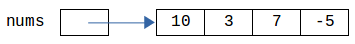
\includegraphics[width=225pt]{array-diagram1.png}
\end{center}


\quest{15 min}


\Q Draw a memory diagram for the following array declarations.

%TODO solution for array memory diagrams
\begin{enumerate}

\item
\begin{javalst}
int[] sizes = new int[5];
sizes[2] = 7;
\end{javalst}

\item
\begin{javalst}
char[] codes = new char[3];
codes[2] = 'X';
\end{javalst}

\item
\begin{javalst}
double[] costs = new double[4];
costs[0] = 0.99;
\end{javalst}

\end{enumerate}


\Q What is the \emph{default} value for uninitialized array elements? (Hint: You should have no empty boxes in your memory diagram.)

\begin{answer}
Zero or equivalent value, depending on the data type.
For numeric types like {\tt int} and {\tt double}, the default is 0; for {\tt boolean}, it's {\tt false}; for {\tt char}, it's {\tt \qs{\bs u0000}\qs}; for reference types, it's {\tt null}.
\end{answer}


\Q Like strings, arrays are reference types. What is the \emph{value} of an array variable?

\begin{answer}
The memory location of the array. If you assign one array variable to another, you're only copying the reference, not the array itself.
\end{answer}


\Q Draw a memory diagram of the following array.
(Hint: You should have four arrows.)

\begin{javalst}
String[] greek = {"alpha", "beta", "gamma"};
\end{javalst}

\begin{answer}
%TODO string array memory diagram
\end{answer}
